\documentclass[]{article}
\usepackage{lmodern}
\usepackage{amssymb,amsmath}
\usepackage{ifxetex,ifluatex}
\usepackage{fixltx2e} % provides \textsubscript
\ifnum 0\ifxetex 1\fi\ifluatex 1\fi=0 % if pdftex
  \usepackage[T1]{fontenc}
  \usepackage[utf8]{inputenc}
\else % if luatex or xelatex
  \ifxetex
    \usepackage{mathspec}
    \usepackage{xltxtra,xunicode}
  \else
    \usepackage{fontspec}
  \fi
  \defaultfontfeatures{Mapping=tex-text,Scale=MatchLowercase}
  \newcommand{\euro}{€}
\fi
% use upquote if available, for straight quotes in verbatim environments
\IfFileExists{upquote.sty}{\usepackage{upquote}}{}
% use microtype if available
\IfFileExists{microtype.sty}{\usepackage{microtype}}{}
\usepackage{graphicx}
\makeatletter
\def\maxwidth{\ifdim\Gin@nat@width>\linewidth\linewidth\else\Gin@nat@width\fi}
\def\maxheight{\ifdim\Gin@nat@height>\textheight\textheight\else\Gin@nat@height\fi}
\makeatother
% Scale images if necessary, so that they will not overflow the page
% margins by default, and it is still possible to overwrite the defaults
% using explicit options in \includegraphics[width, height, ...]{}
\setkeys{Gin}{width=\maxwidth,height=\maxheight,keepaspectratio}
\ifxetex
  \usepackage[setpagesize=false, % page size defined by xetex
              unicode=false, % unicode breaks when used with xetex
              xetex]{hyperref}
\else
  \usepackage[unicode=true]{hyperref}
\fi
\hypersetup{breaklinks=true,
            bookmarks=true,
            pdfauthor={},
            pdftitle={},
            colorlinks=true,
            citecolor=blue,
            urlcolor=blue,
            linkcolor=magenta,
            pdfborder={0 0 0}}
\urlstyle{same}  % don't use monospace font for urls
\setlength{\parindent}{0pt}
\setlength{\parskip}{6pt plus 2pt minus 1pt}
\setlength{\emergencystretch}{3em}  % prevent overfull lines
\setcounter{secnumdepth}{5}


\begin{document}

%  Titelblad

% Opmerking: gaat uit van een \baselinestretch waarde van 1.5 (die moet
% ingesteld worden voor het begin van de document endvironment)

\begin{titlepage}

\setlength{\hoffset}{-0.3in}
\setlength{\voffset}{-1in}
\setlength{\topmargin}{1.5cm}
\setlength{\headheight}{0.5cm}
\setlength{\headsep}{1cm}
\setlength{\oddsidemargin}{3cm}
\setlength{\evensidemargin}{3cm}
\setlength{\footskip}{1.5cm}
\enlargethispage{1cm}
% \textwidth en \textheight hier aanpassen blijkt niet te werken

\fontsize{12pt}{14pt}
\selectfont

\begin{center}


\includegraphics[height=2cm]{logo.png}

\vspace{0.5cm}

Universidad Sim\'on Bol\'ivar\\
Departamento de computaci\'on\\
Miniproyecto de Desarrollo de Software EP4793\\

\vspace{3.5cm}

\fontseries{bx}
\fontsize{17.28pt}{21pt}
\selectfont

Desarrollo de procesador de horarios \\
para la coordinación de computación\\


\fontseries{m}
\fontsize{12pt}{14pt}
\selectfont

\vspace{.6cm}



\vspace{.4cm}


\vspace{3cm}

Tutores : \\
Eduardo Blanco\\
Carolina Mart\'inez\\
\vspace{1cm}
Alumno: \\
Daniel  Leones \\


\vspace{1cm}

7 de diciembre del 2016

\end{center}
\end{titlepage}

{
\hypersetup{linkcolor=black}
\setcounter{tocdepth}{3}
\tableofcontents
}

\newpage
\section{Introducción}\label{introducciuxf3n}

La coordinación de ingeniería de la computación realiza diversas tareas
tanto académicas como administrativas. Una de ellas es la preparación,
emisión y publicación de horarios para trimestres posteriores al actual.
Luego, ante los estudiantes y a DACE (Dirección de Administración y
Control de Estudios).

Durante las semanas finales de cada trimestre, la coordinación debe
preparar y emitir la oferta de asignaturas. Los insumos para poder
realizar el análisis de horarios se encuentra en diversos estilos de
presentación y en al menos tres tipos de archivos. Por otra parte, no se
emite una única oferta sino que se realizan varias revisiones de la
misma debido a que DACE, realiza ajustes y correcciones de ella lo cual
obliga a la coordinación a volver a repetir el proceso de preparación y
emisión.

Este proceso es realizado de forma manual. Dado que es necesario
contrastar mucha información, es muy propenso a errores lo cual afecta
la publicación fidedigna de las materias disponibles. La coordinadora
realiza este proceso ante la falta de un asistente pero debe emplear
mucho tiempo en los preparativos y el análisis.

En este miniproyecto de desarollo se analiza y se pretende solucionar
este problema mediante la automatización del proceso. La implantación
del programa se realizó en el lenguaje de programación Python y fue
diseñada para ser utilizada en entornos de tipo Unix. No obstante, esto
no impide que sea utilizada en otros entornos dada la característica
multiplataforma de Python.

En este informe, se observa el problema a plenitud, estructura, diseño e
implantación de la aplicación que automatiza esta tarea administrativa
y, pruebas y resultados de la solución.

\section{Resumen}\label{resumen}

Una de las tareas de la coordinación de ingenieria de la computación,
durante cada trimestre, es la preparación, emisión y publicación de los
horarios de los trimestres posteriores al actual. Para realizar esta
tarea, se requiere de las ofertas departamentales y una preoferta 0800.
Se analiza cada oferta de los departamentos que tengan materias que
correspondan al pensum de ingenieria de la computación contra la
preoferta 0800. Se genera una primera preoferta que se envía a DACE
(Dirección de Administración y Control de Estudios). Luego, esta
preoferta se somete a continuos análisis, es decir, repetir la
preparación cada vez que existen ajustes y/o correcciones por parte de
DACE, hasta que no existan más. Finalmente, se publica a los
estudiantes.

Este proceso es realizado de forma manual; la coordinadora es la única
persona que puede hacerlo dada la carencia de un asistente relacionado
con estas labores; es propenso a errores debido a la cantidad de
información que una sola persona debe manejar. Estos factores implican
que la preparación tome mucho tiempo.

En este miniproyecto, se diseñó e implantó con éxito una aplicación que
automatiza y soluciona este problema con ciertas condiciones.
Concretamente, se implantó procesadores de texto para documentos DOC,
XLS y PDF como la base la aplicación; luego, se construyó una aplicación
principal que realiza las emisiones de ofertas bajo determinadas reglas
de la coordinación.

Se realizaron 32 casos de prueva en total, que consiste en: dos de
propósito de la aplicación y el resto en pruebas de procesamiento de
texto. Un caso de prueba importante fue realizar la preparación y
emisión de la oferta del trimestre enero-marzo 2017.

\section{Planteamiento del problema}\label{planteamiento-del-problema}

Trimestralmente la coordinación de ingenieria de la computación prepara,
emite y publica a DACE las ofertas de materias, de acuerdo al pensum
vigente, para los posteriores trimestres.

Las ofertas de materias consisten en asignaturas que los departamentos
proporcionan a cada carrera dentro de la universidad de acuerdo al
pensum. Lo anterior se denominan ofertas departamentales. Las tales se
presentan bajo diferentes formatos y archivos; hasta ahora se conocen
que los archivos entregados son PDF, DOC, XLS (Excel) y XLSX. Por otra
parte, las ofertas son escritas de acuerdo a ciertos estilo de
presentación de la información que varia entre departamentos. Cada
oferta consiste en renglones compuestos de:

\begin{itemize}
\itemsep1pt\parskip0pt\parsep0pt
\item
  código de asignatura
\item
  bloque
\item
  horario.
\end{itemize}

Cada renglón debe ser examinado contra un borrador de ofertas que la
coordinación dispone; en cada caso se agrega, elimina o modifica su
inclusión al borrador. Luego de este examen, se produce un borrador
tentativo se que envia a DACE.

Sin embargo, la oferta producida no se da por terminada ya que está
sujeta a varias revisiones conforme DACE la dicte. Esto significa que el
proceso anteriormente descrito se repita hasta que no hayan nuevas
versiones por parte de DACE.

Todo el proceso anteriormente descrito es realizado de forma manual por
la coordinación. Es propenso a cometer errores debido a la cantidad de
información que se debe analizar y comparar. Esto afecta en la
publicación fidedigna de la oferta de asignaturas. Ante la falta de un
asistente, la coordinadora es la persona encargada de realizar este
trabajo el cual consume una buena parte del tiempo en su preparación y
revisión.

\section{Objetivos}\label{objetivos}

\begin{itemize}
\item
  Implementación de una aplicación que permita la integración de los
  horarios de las asignaturas enviados por los distintos departamentos.
\item
  Analizar, modificar e integrar ofertas provenientes de los diferentes
  departamentos que ofertan materias a la coordinación de ingeniería de
  la computación.
\item
  Facilitar y automatizar la gestión de los horarios en los trámites
  académicos de la coordinación.
\end{itemize}

\section{Análisis}\label{anuxe1lisis}

El flujo de trabajo del procesador de horarios es similar al proceso
expuesto en el planteamiento del problema. Es modelado por dos etapas
con sus constituyentes:

\begin{itemize}
\itemsep1pt\parskip0pt\parsep0pt
\item
  \textbf{Etapa 1}:

  \begin{itemize}
  \itemsep1pt\parskip0pt\parsep0pt
  \item
    Ofertas departamentales, oferta 0800 y diccionario de materias.
  \item
    Análisis y comparación.
  \item
    Emisión de preoferta a DACE
  \end{itemize}
\item
  \textbf{Etapa 2:}

  \begin{itemize}
  \itemsep1pt\parskip0pt\parsep0pt
  \item
    Análisis y comparación con nueva oferta de DACE.
  \item
    Generación de oferta trimestral.
  \end{itemize}
\end{itemize}

\subsection{Etapa 1}\label{etapa-1}

En esta etapa, se reune todas las ofertas departamentales y una
preoferta 0800 como alimentación al procesador. Luego, éste produce una
oferta a DACE que se usará para la etapa 2.

%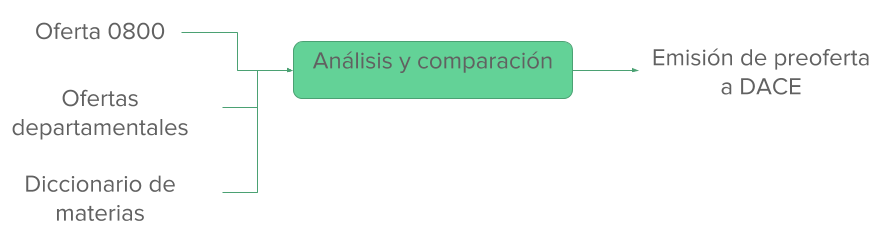
\includegraphics{primera_etapa.png} \textbf{Figura:} primera etapa.

\begin{figure}[!h]
  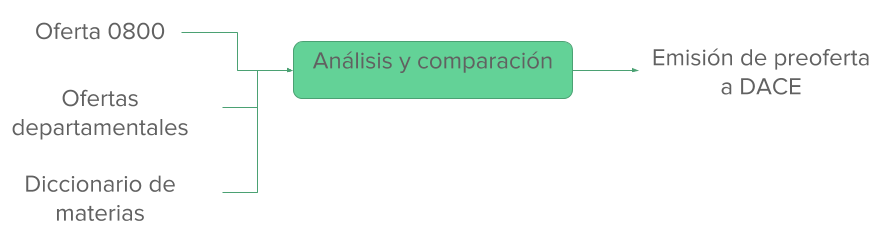
\includegraphics[width=\linewidth]{primera_etapa.png}
  \caption{Primera etapa}
  \label{fig:primera_etapa}
\end{figure}

\textbf{Ofertas departamentales:} en cada trimestre, los departamentos
entregan las ofertas de asignaturas en archivos con formatos diversos.
Los formatos conocidos hasta ahora son: XLS (Excel), XLSX, PDF y DOC.
Estas ofertas son generales, es decir, cada coordinación de carrera
extrae y analiza la información relevante a su dominio. Todos las
archivos departamentales se utilizan como insumo para generar una
primera oferta. Las materias que sean pertinentes a la coordinación se
seleccionan a través del diccinario de materias.

El formato de presentación de las asignaturas varia en cada
departamento. Existen 2 formatos comunes, aunque no necesariamente en el
orden descrito. He aqui los siguientes:

\begin{itemize}
\itemsep1pt\parskip0pt\parsep0pt
\item
  Código, Nombre Asignatura, Bloque, Lunes, Martes, Miercoles, Jueves,
  Viernes, Carrera
\item
  Códigos, Asignaturas, horarios.
\end{itemize}

\textbf{Oferta 0800:} Archivo contra el cual se comparan las ofertas de
los departamentos. Suele estar en formato XLS (Excel). Este archivo es
el primer insumo requerido para generar una primera oferta.

El formato del archivo es el siguiente y sigue el orden descrito:

\begin{itemize}
\itemsep1pt\parskip0pt\parsep0pt
\item
  Código, Bloque, Lunes, Martes, Miercoles, Jueves, Viernes, Oferta
  Especial, Carrera, Operación.
\end{itemize}



\textbf{Análisis y comparación:} Las ofertas departamentales y la 0800
son analizadas y comparadas bajo ciertas reglas y se genera una oferta
preliminar. Basta decir, que la comparación consiste eliminar y agregar
asignaturas, y modificar el horario en el caso que haya discrepancias.
Más adelante, se discuten las reglas de comparación.

\textbf{Emisión preliminar de materias a DACE:} el resultado es un
archivo en formato CSV (siglas en inglés, comma-separated value) bajo el
siguiente orden:

\begin{itemize}
\itemsep1pt\parskip0pt\parsep0pt
\item
  Código, Bloque, Lunes, Martes, Miercoles, Jueves, Viernes, Especial,
  Carrera, Operación
\end{itemize}

\textbf{Diccionario de materias:} es un archivo de texto donde se
enuncian los códigos de las asignaturas. Se utiliza para discriminar las
materias relevantes a la coordinación. Tiene la siguiente estructura:

\begin{verbatim}
# Comentarios para clasificar las materias 
código1
codigo2
...
# Comentarios para clasificar las materias 
codigo4
...
codigo6
\end{verbatim}

Los comentarios son opcionales y por razón de legibilidad del archivo.

\subsection{Etapa 2}\label{etapa-2}

Para esta etapa se utiliza el producto de la etapa 1, es decir, la
preoferta. La salida es una oferta trimestral final; siempre y cuando no
hayan cambios por parte de DACE.

\begin{figure}[!h]
  
\includegraphics[width=\linewidth]{segunda_etapa.png}
  \caption{Segunda etapa}
  \label{fig:segunda_etapa}
\end{figure}
%
\includegraphics{segunda_etapa.png} \textbf{Figura:} segunda etapa.

\textbf{Análisis y comparación con nueva oferta de DACE:} una vez que se
haya producido una primera oferta, se debe reanalizar y comparar contra
la oferta general de DACE. Tal documento se reproduce en formato PDF; en
él, se encuentra, para cada carrera de la universidad, sus asignaturas
para el trimestre posterior. La comparación consiste en eliminar y
agregar asignaturas, y modificar el horario en el caso que haya
discrepancias. Más adelante, se discuten las reglas de comparación.


\begin{figure}[!h]
  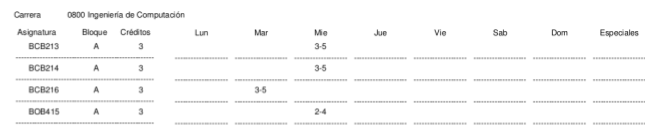
\includegraphics[width=\linewidth]{ejemploDACE.png}
  \caption{Ejemplo de lista general de DACE.}
  \label{fig:lista_general_dace}
\end{figure}

\textbf{Generación de oferta trimestral:} para esta etapa se genera un
borrador de materias para entregar a DACE. No obstante, esta sujeto a
cambios mientras haya revisiones de la oferta general de DACE. Esto
significa que, el producto de esta etapa debe volver a pasar por la
etapa anterior; generar una nueva oferta hasta que no hayan nuevas
revisiones.

El formato de esta etapa será en CSV con la siguiente presentación:

\begin{itemize}
\itemsep1pt\parskip0pt\parsep0pt
\item
  Código, Bloque, Lunes, Martes, Miercoles, Jueves, Viernes, Oferta
  Especial, Carrera, Operación.
\end{itemize}

\subsection{Especificación de reglas}\label{especificaciuxf3n-de-reglas}

En los archivos de salida de las dos etapas, una fila $x$ consiste en

$x = (cod1,bloque1,horarios,especial,carrera,operación)$

donde

\begin{itemize}
\item
  $horarios$: son las posiciones de los dias en el siguientes orden:
  Lunes, Martes, Miercoles, jueves, viernes. En tales espacios son los
  horas.
\item
  $operación$: los valores son M(modificado), E(eliminar) , I(insertar)
  o vacio (en el archivo puede verse que no hay datos en tal campo).
\end{itemize}

Las reglas de comparación se aplican a todos los campos de la fila x
salvo en $carrera$ y $operación$. En el campo de $operación$ se anota el
resultado de aplicar alguna regla.

Para la primera etapa, existen 3 reglas de comparación. Sea A un archivo
de ofertas de DACE y B cada una de las ofertas departamentales: 
\begin{itemize}
\item
  Si fila de A y B son iguales en sus campos, el resultado es vacio. En caso
  contrario, se escribe la fila de A como resultado, el resultado es M.

\item
  Si una fila de A no existe en B, su operación es E. Se escribe en el
  archivo final.
\item
  Si una fila de B no existe en A, su operación es I. Se escribe en el
  archivo final.
\end{itemize}

Para la segunda etapa, existen 3 reglas de comparación y se apoyan en
los resultados de la primera etapa. Sea A un archivo CSV de la primera
etapa y B un archivo de ofertas general de DACE:

\begin{itemize}
\item
  Si una fila de A con operación M, es no igual en sus campos a una de
  B, se escribe la fila de A.
\item
  Si una fila de A con operación E, no existe en B, se escribe la fila
  de B.
\item
  Si una fila de A con operación es I, no existe en B, se escribe la
  fila de A.
\item
  Si una fila de A con operación vacia no existe en B, se escribe la
  fila de A con operación I. Por otra parte, si se encuentra y no son
  iguales sus campos, se agrega la fila de A con operación M.
\end{itemize}

\section{Diseño e implantación}\label{diseuxf1o-e-implantaciuxf3n}

La implantación del procesador de horarios se realizó con el lenguaje de
programación Python versión 3.4. Sin embargo, no existe incompatibilidad
en versiones posteriores.

Las dependencias externas a la biblioteca estandar de Python son las
siguientes:

\begin{itemize}
\itemsep1pt\parskip0pt\parsep0pt
\item
  Libreoffice
\item
  PyMupdf
\item
  xlrd
\end{itemize}

\subsection{Arquitectura}\label{arquitectura}

El procesador de horarios consta de 6 módulos. Tres módulos se encargan
de la lectura de las ofertas departamentales a saber:
\texttt{procesadorDOC}, \texttt{procesadorXLS}, \texttt{procesadorPDF}.
El \texttt{procesadorDACE} espera un archivo PDF que contenga el formato
que se observa en la imagen de abajo. El módulo de
\texttt{funcionesAuxiliares} contiene funciones de apoyo a los
procesadores anteriores. El \texttt{procesadorOfertas} es el programa
principal y donde reside la lógica del sistema. El script
\texttt{procesadorOfertas.sh} se utiliza para abstraer detalles de
ejecución, detectar errores y automatizar la conversión de archivos DOC
a FODT(XML de libreoffice).

\begin{figure}[!h]
  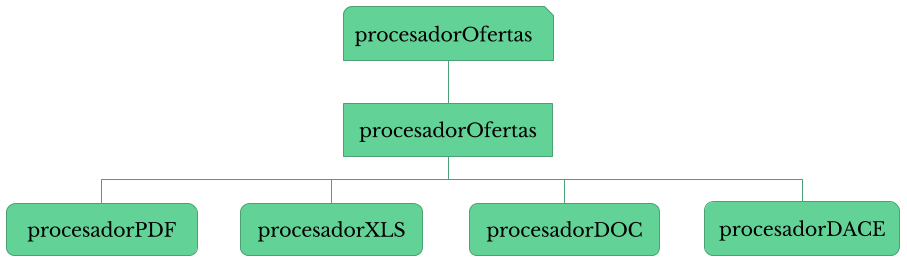
\includegraphics[width=\linewidth]{Estructura.png}
  \caption{Arquitectura del procesador de horarios.}
  \label{fig:arquitectura_procesador}
\end{figure}

% 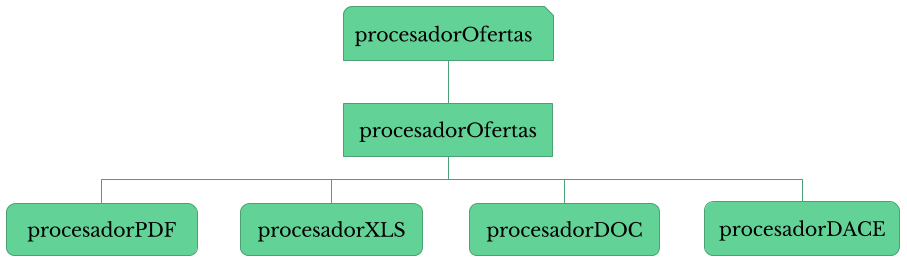
\includegraphics{Estructura.png} \textbf{Figura:} Arquitectura del
% procesador de horarios

\subsubsection{Captura de datos}\label{captura-de-datos}

Debido a la diferencias de formatos, dificultades de reconocimiento y
estilos en como se presenta la información, los procesadores pueden
reconocer datos, de acuerdo, a dos estilos a saber:

\begin{itemize}
\item
  \textbf{Estilo general:} Código, Nombre Asignatura, Bloque, Lunes,
  Martes, Miercoles, Jueves, Viernes, Carrera.

  Sólo cualquier otro campo adicional se omitirá y sólo se relevante
  para el procesador los siguientes: código, bloque, lunes, martes,
  miercoles, jueves, viernes y, opcionalmente, carrera.

  Los módulos \texttt{procesadorPDF} y \texttt{procesadorXLS} fueron
  diseñados para reconocer este estilo. No obstante, procesadorXLS puede
  reconocer, adicionalmente, un campo denominado \texttt{especiales}.
\item
  \textbf{Estilo departamento de computo:} Códigos, Bloques o sección,
  horarios. Los \texttt{bloques} pueden aparecer en \texttt{Códigos} o
  no existir.

  El \texttt{procesadorPDF} y el \texttt{procesadorDOC} pueden manejar
  estos estilos.
\end{itemize}

\subsection{Ejecución}\label{ejecuciuxf3n}

El procesador de horarios se ejecuta utilizando la linea de comando, a
través del interprete de Python o haciendo uso del script para sistemas
tipo Unix. Se recomienda usar el script \texttt{.sh}.

Para ayudar familiarizarse con la ejecución, la aplicación dispone de
una opción de ayuda usando la opción -h como sigue:

\texttt{procesadorOferta.sh -h}

Además, se escribió un documento de ayuda para instalar, configurar y
ejecutarla. Se encuentra entre los archivos de la aplicación.

Para ejecutar la aplicación se escribe lo siguiente:

\begin{itemize}
\itemsep1pt\parskip0pt\parsep0pt
\item
  \textbf{Primera etapa:}
\end{itemize}

\texttt{procesadorOferta.sh -e directorio/a/insumos -d preoferta\_0800.xls      -f directorio/a/archivo\_de\_salida.csv -m archivo\_diccionario\_materias}

Al usar \texttt{-d} y \texttt{-m} se asume que estos archivos están en
el directorio de insumos.

\begin{itemize}
\itemsep1pt\parskip0pt\parsep0pt
\item
  \textbf{Segunda etapa:}
\end{itemize}

\texttt{procesadorOferta.sh -r -d oferta\_dace.pdf      -f directorio/a/archivo\_de\_salida.csv      directorio/a/archivo\_de\_preoferta.csv}

\subsection{Pseudocódigos}\label{pseudocuxf3digos}

El procesadorPDF procesa un archivo PDF de la siguiente manera:

\begin{verbatim}
    archivoXML = pdf2xml(archivoPDF)
    while (!eof(archivoXML))
        linea = archivoXML.leerLinea()
        if !cabeceraLista
            cabeceraLista = analizarCabecera(linea)
        else
            listaMatBloq.anexar(extraerCodMat(linea))
            listaMatBloq.anexar(extraerBloque(linea))
            listaHorarios.anexar(extraerHorarios(linea))

    foreach fila in listaMatBloq
        Componer fila con horarios respectivos.
        if (fila.Cod_mat no esta la lista de materias requeridas)
            Eliminar fila
        listaOfertas.anexar(fila)

    foreach fila in listaOfertas
        filaCSV = fila_a_csv(fila)
        salida.escribir(filaCSV)
\end{verbatim}

El procesadorDOC procesa un archivo FODT, producto de una función de
\texttt{libreoffice.}

\begin{verbatim}
    while (!eof(archivoFODT))
        linea = archivoFODT.leerLinea()
        codMat = extraerCodMat(linea)
        bloq = extraerBloque(linea)
        hor = extraerHorarios(linea)
        especiales = extraerEspeciales(linea)
        fila = [codMat,bloq,hor,especiales]
        if (fila.Cod_mat no esta la lista de materias requeridas)
            Eliminar fila
        filaCSV = fila_a_csv(fila)
        salida.escribir(filaCSV)
\end{verbatim}

El procesadorXLS procesa un archivo XLS mediante la dependencia xlrd.

\begin{verbatim}
    foreach fila in archivoXLS.
        if !cabeceraLista
            cabeceraLista = analizarCabecera(linea)
        else
            if (fila.Cod_mat no esta en lista de materias requeridas
            || fila.Carrera != '0800')
            continue

        filaCSV = fila_a_csv(fila)
        salida.escribir(filaCSV)
\end{verbatim}

Para generar una primera oferta trimestral, esto es, la primera etapa:

\begin{verbatim}
    listaMaterias = cargarMateriasRequeridas()
    (listasOfertas, listaDaCE) = cargarOfertas
                            (args,dirBase,listaMaterias,nomArchDace)
    primeraOferta = generarOferta(listaOfertas,listaDACE)
    escribirResultados(primeraOferta,archSalida)
\end{verbatim}

Para generar ofertas trimestrales contra un listado de DACE, esto es, la
segunda etapa:

\begin{verbatim}
    listaOfertas = cargarOfertaPrimera(nombreArchivoOferta)
    listaGenDace = cargarListaGeneralDace(nombreArchivoDacePDF)
    resultado = analizarComparar(listaOfertas,listaGenDace)
    resultadoCSV = a_CSV(resultado)
    salida.escribir(resultadoCSV)
\end{verbatim}

\section{Plan de pruebas y
resultados}\label{plan-de-pruebas-y-resultados}

Para evaluar la capacidad del procesador de horarios, se realizaron
pruebas en los siguientes ambitos:

\begin{itemize}
\item
  \textbf{Procesamiento de formato:} se evalúa la capacidad de captura
  de datos de los procesadores. Esto son: procesadorDACE, procesadorDOC,
  procesadorPDF, procesadorXLS.
\item
  \textbf{Procesamiento de primera etapa:} se evalúa la salida del
  programa para la primera etapa. Se espera que el programa analice y
  etiquete cada ofertas en función de las operaciones: E, I, M.
\item
  \textbf{Procesamiento de segunda etapa:} se evalúa la salida del
  programa para la segunda etapa. Se espera que el programa reuna las
  materias correctas para un trimestre determinado.
\end{itemize}

\subsection{Procesamiento de formato}\label{procesamiento-de-formato}

Los casos de pruebas son archivos que corresponda a cada procesador.
Estos casos fueron elaborados de la siguiente manera:

\begin{itemize}
\item
  \textbf{Archivos con datos ficticios:} fueron diseñados para ejercitar
  las capacidades del procesador en cuestión. La información fue tomada
  de los archivos reales con ligeras variaciones.

  Se presentan con la nomenclatura: \textgreater{} docX.{[}extensión{]}
  \textgreater{} donde X: es el numero del caso de prueba.

  Si hay 3 versiones de formato de un mismo doc, entonces la validación
  es la misma para todos; por ejemplo, si existen doc1.pdf, doc1.xml y
  doc1.xls, la información reconocida, pese a la diferencias de
  formatos, es igual para todas.
\item
  \textbf{Archivos con datos reales:} se usan para validar la
  información y para verificar reconocimiento de patrones de
  información.
\end{itemize}

\subsection{Procesamiento de primera etapa y segunda
etapa}\label{procesamiento-de-primera-etapa-y-segunda-etapa}

Se utilizan los archivos de ofertas trimestrales facilitados por la
coordinación de computación. Existen dos casos de pruebas:

\begin{itemize}
\item
  \textbf{SD2016:} Se usaran las ofertas departamentales, la preoferta
  0800 a Dace del trimestre septiembre-diciembre 2016.
\item
  \textbf{EM2017:} Se usaran las ofertas departamentales, la preoferta
  0800 a Dace del trimestre enero-marzo 2017.
\end{itemize}

Para la segunda etapa, se usa la lista general de DACE para tal periodo.

\section{Conclusión}\label{conclusiuxf3n}

El procesador de horarios fue implantado exitosamente para cubrir los
formatos y archivos planteados anteriormente. No obstante, queda el
problema cuando los formatos de archivos y/o estilos de ofertas
departamentales cambien. Para el caso de formatos de archivos, el
procesador se puede extender fácilmente y adaptarse al módulo principal.
Por otra parte, si cambian los estilos se hará necesario implementar
nuevos reconocimientos sin descartar los que se hayan implementado. El
\texttt{procesadorXLS} es el reconocedor más flexible para cambios en
cuanto estilos de presentación de la información.

En cuanto a las pruebas, se realizaron 20 casos de pruebas de
procesamiento: 12 para casos con datos ficticios y 7 usando datos reales
de la coordinación. Se realizaron 3 pruebas para primera etapa y 2 para
la segunda etapa. Una de las pruebas consistió en generar la oferta del
trimestre Enero-Marzo 2017 para ambas etapas.

\section{Apéndice}\label{apuxe9ndice}

\subsection{Casos de pruebas con datos ficticios creados para
procesamiento}\label{casos-de-pruebas-con-datos-ficticios-creados-para-procesamiento}

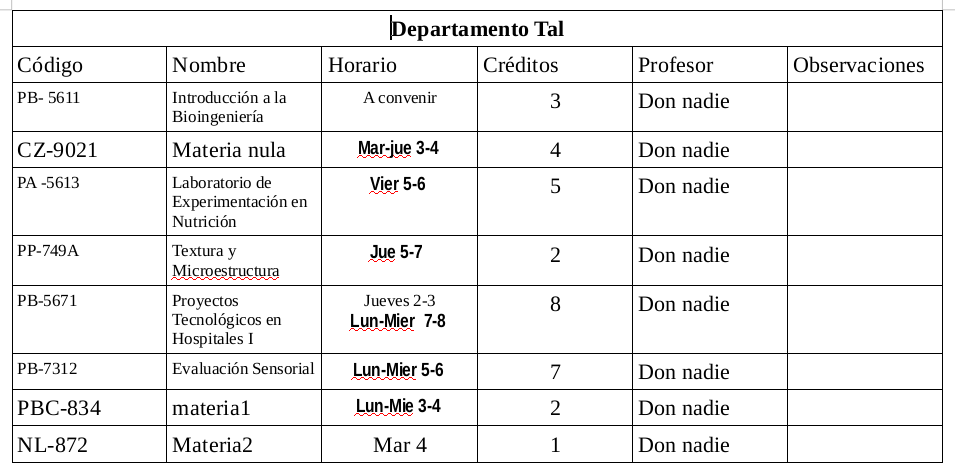
\includegraphics{casos_pruebas/doc1DOC.png} \textbf{Figura:} Reconocer
materias sin horario. Versión DOC.

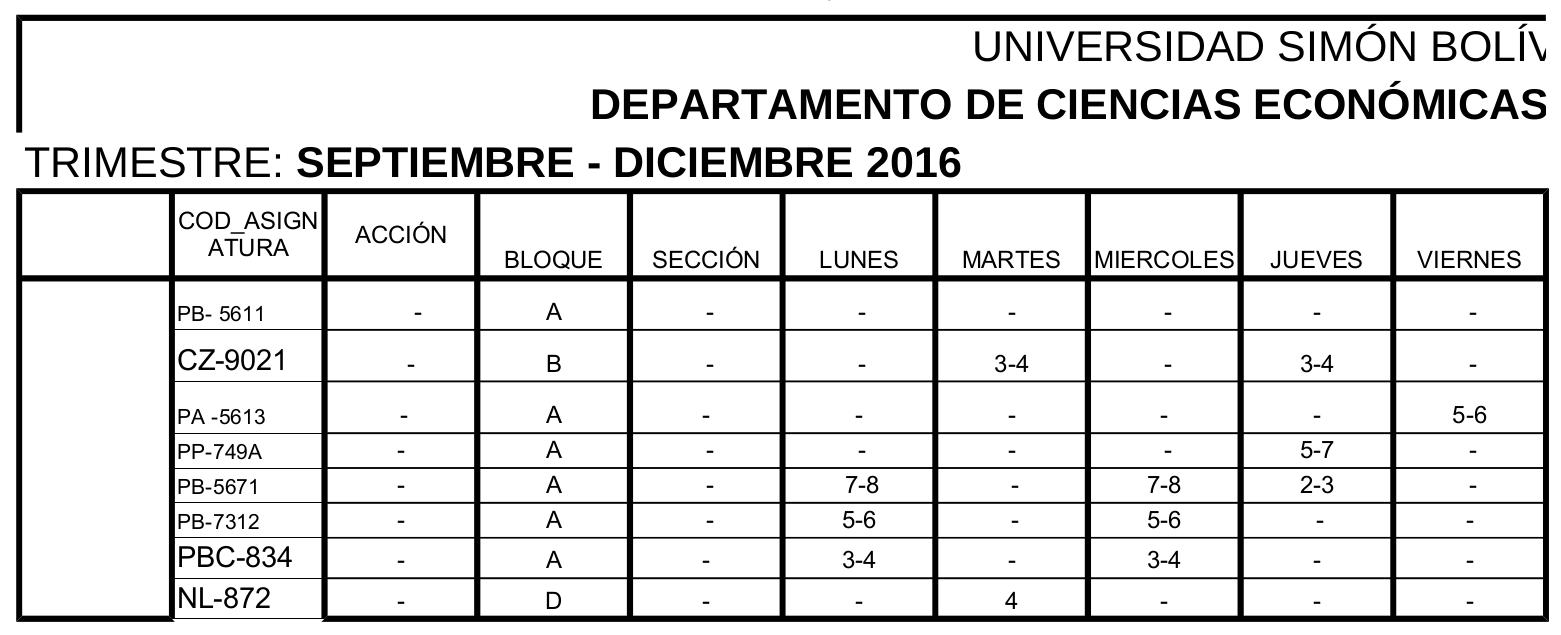
\includegraphics{casos_pruebas/doc1PDF.png} \textbf{Figura:} Reconocer
materias sin horario. Versión PDF.

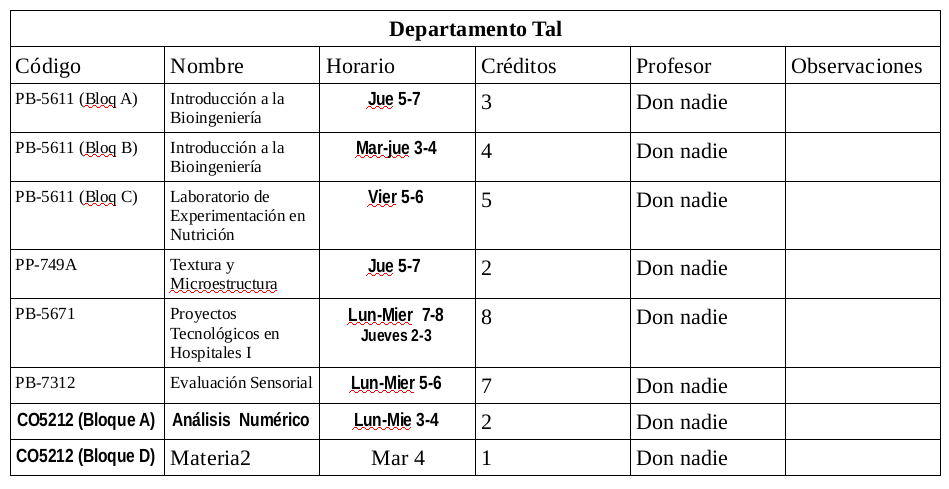
\includegraphics{casos_pruebas/doc2DOC.png} \textbf{Figura:} Reconocer
materias con varias secciones y una hora. Versión DOC.

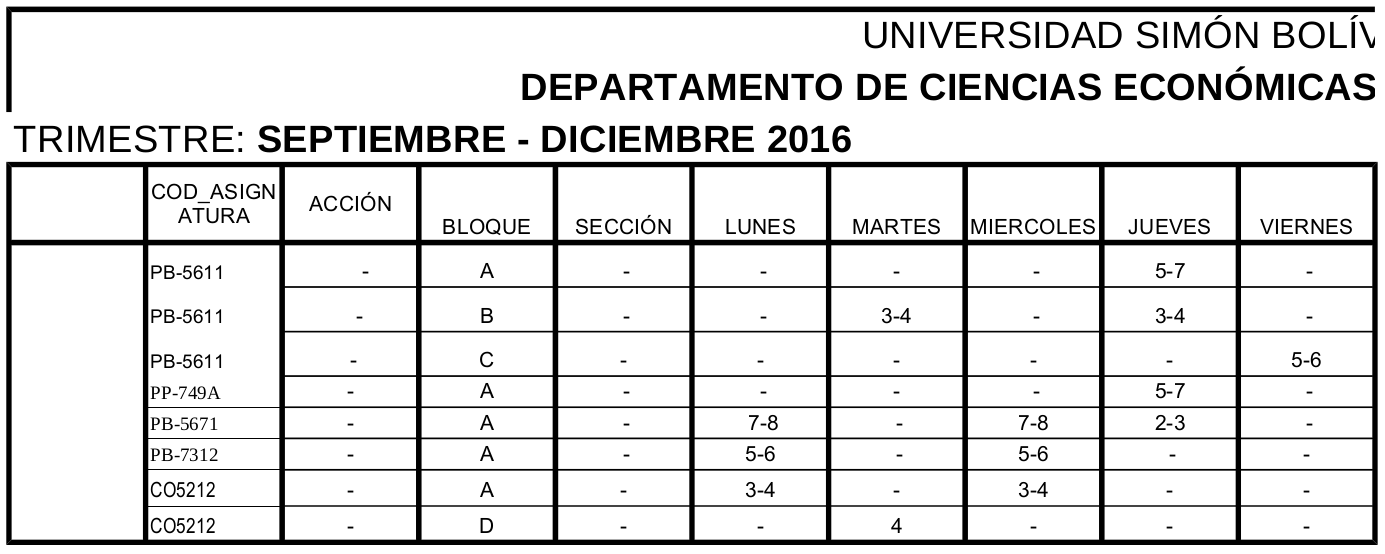
\includegraphics{casos_pruebas/doc2PDF.png} \textbf{Figura:} Reconocer
materias con varias secciones y una hora. Versión PDF.

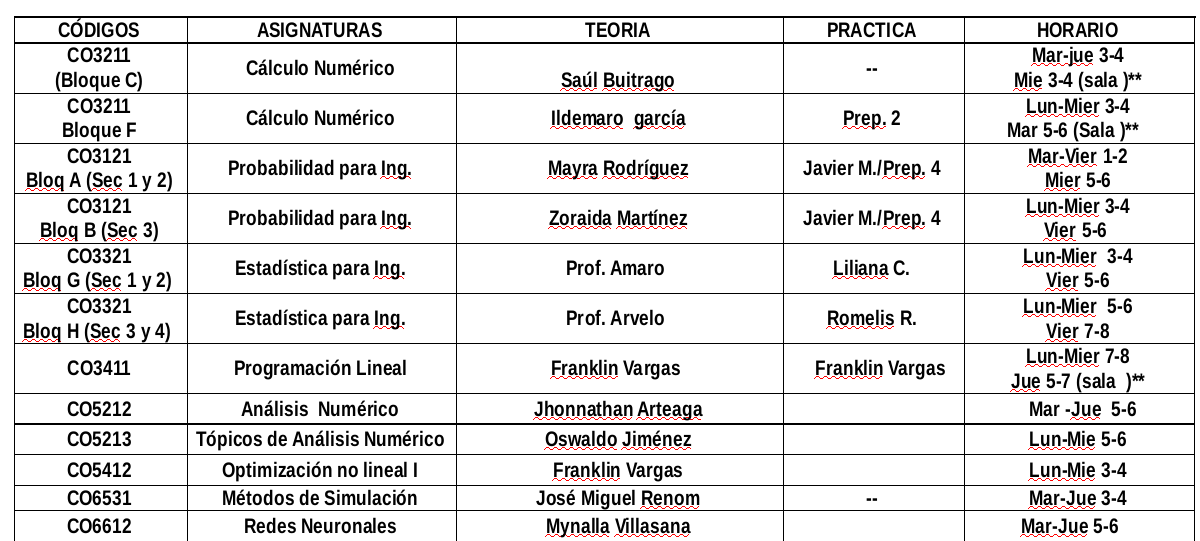
\includegraphics{casos_pruebas/doc3DOC.png} \textbf{Figura:} horarios
desorganizados y reconocimiento de todas las materias.

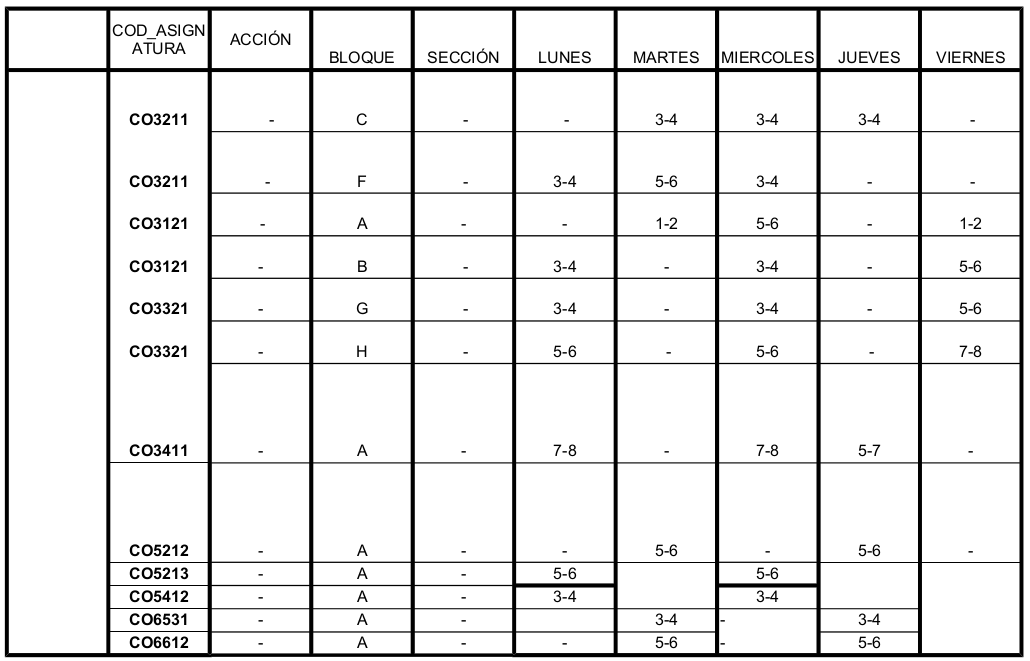
\includegraphics{casos_pruebas/doc3PDF.png} \textbf{Figura:}
reconocimiento de todas las materias

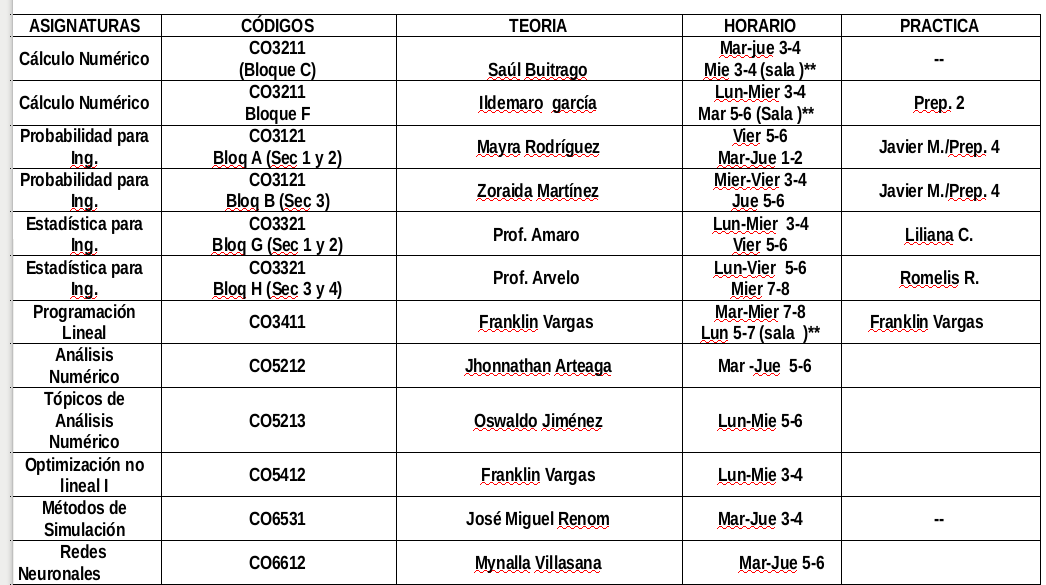
\includegraphics{casos_pruebas/doc4DOC.png} \textbf{Figura:} orden de
los campos cambiados. Versión PDF.

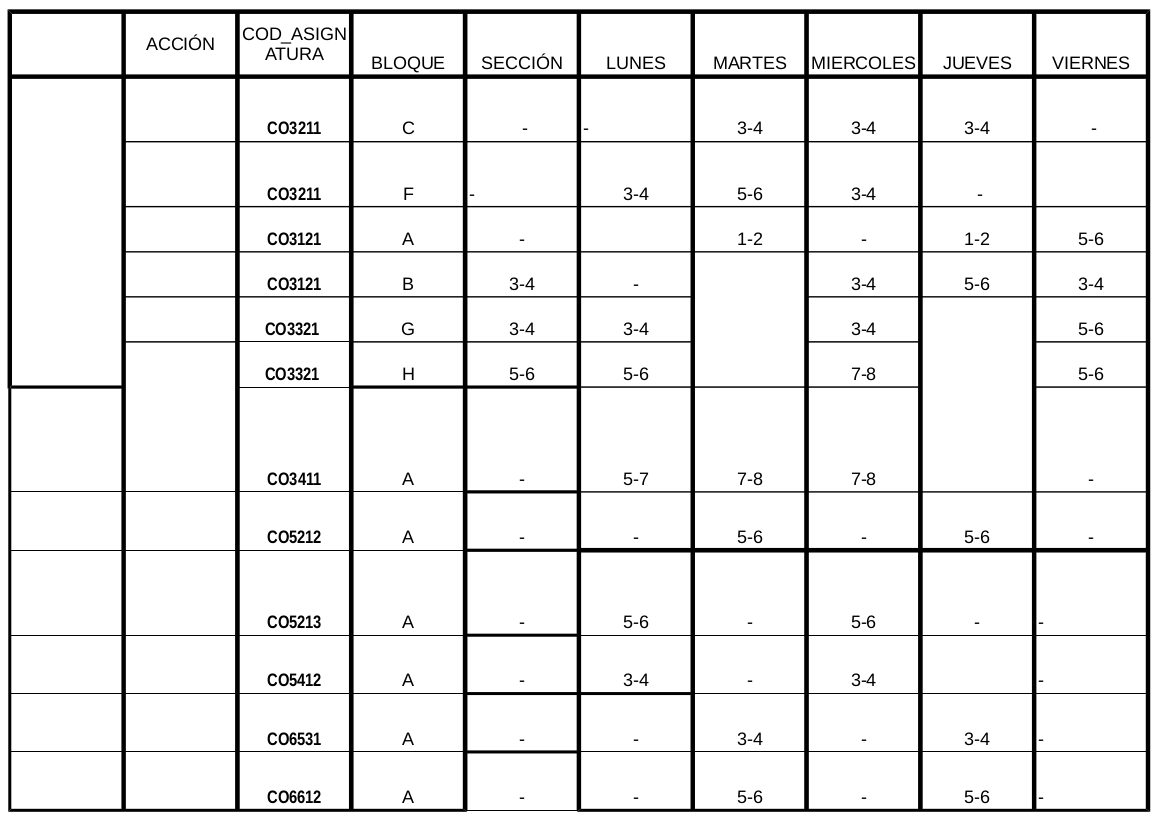
\includegraphics{casos_pruebas/doc4PDF.png} \textbf{Figura:} orden de
los campos cambiados.

\section{Anexos}\label{anexos}

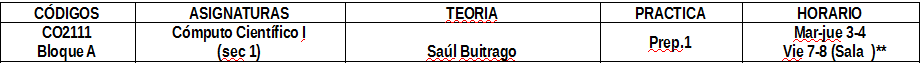
\includegraphics{Insumos2.png} \textbf{Figura:} Estilos de oferta del
cepartamento de cómputo.

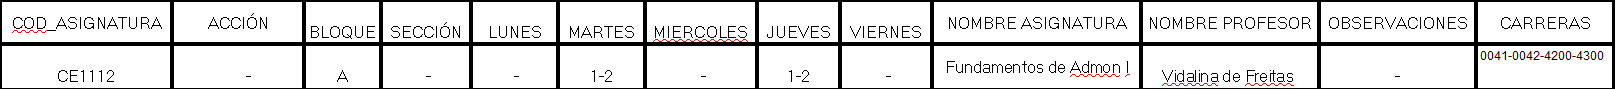
\includegraphics{Insumos.png} \textbf{Figura:} Estilo de ofertas del
departamento de ciencias ecónomicas.

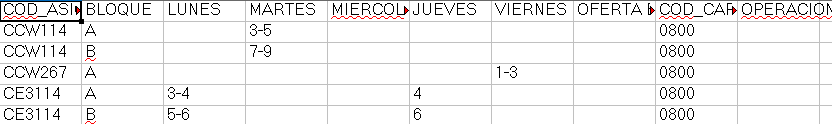
\includegraphics{muestra_dace.png} \textbf{Figura:} Estilo de oferta de
la lista de ofertas de DACE.

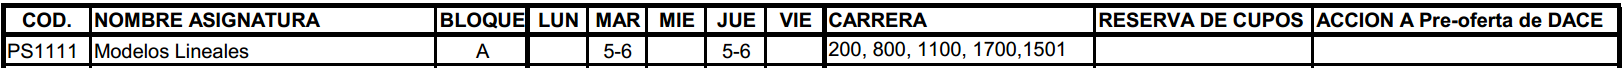
\includegraphics{Insumos3.png} \textbf{Figura:} Estilo de ofertas del
departamentos de sistemas.

\section{Bibliografía}\label{bibliografuxeda}

\href{https://github.com/python-excel/tutorial}{Repositorio de XLRD}

\href{http://xlrd.readthedocs.io/en/latest/}{Documentación de XLRD}

\href{https://github.com/javierlopm/sistemaPermisosComputacion}{Repositorio
del procesador de horarios}

\href{http://pythonhosted.org/PyMuPDF/installation.html}{Documentación
de pyMuPDF}

\end{document}
